\section{Infrastructure: Utilities}
\label{sec:utilclasses}

\subsection{Introduction}

The previous infrastructure section described the data handling 
objects in ESMF. This section describes the lowest level
objects in the infrastructure layer, the utility classes.
Some of these methods will be called directly by user-supplied
code; others are intended to provide support for internal ESMF 
code.

\subsection{Design Goals and Considerations}

One of the goals of the utility layer is to present a uniform interface
for common system functions.  Hardware platforms often have
different system libraries and methods for accomplishing what are 
logically the same tasks.  Routines in this layer insulate user code 
from these variations so that it is portable from system to system.  

In most cases these utilities occupy the lowest level of the object hierarchy.
Another advantage of isolating them is to help avoid circular referencing.

An important goal of the utility layer is to enhance performance portability and
ease of use by establishing structured machine and programming models.  
The machine model captures the performance critical features of a computing 
platform, encoding information about the hardware configuration in a 
systematic way so that it can be analyzed and manipulated.  The programming
model uses this encoded information to allow the user to create
optimized decompositions using a simple, abstract interface.  More detail
on the progaramming model is presented in Section~\ref{sec:progmodel}.

\subsection{Programming Model}
\label{sec:progmodel}

The ESMF programming model defines abstractions that expose
features of the computing environment to the user.  It must support the 
efficient utilization of system resources such as   
computing hardware, OS, and standard library or vendor-supplied 
software (e.g., MPI or other message-passing software, Posix threads, OMP),
and must present a reasonably simple interface to the application 
developer.  

ESMF abstracts the compute elements over which data and tasks may be
distributed into decomposition elements, or {\tt DE}s, which
are essentially threads.  For MPP architectures in which there
is tyically one thread per process, the {\tt DE} degenerates to a 
process.
Depending on the hardware system, ESMF threads will be to a limited 
extent compatible with user-defined threads.  The user will have 
the option to enable ESMF threading or not.  In the latter case, the
{\tt DE} again degenerates to a process.

{\tt DE}s are organized into topologies, such as a 2D grid, by the 
{\tt Layout} 
class.  A user can create a {\tt Layout} directly, or a {\tt Layout} can be 
constructed automatically in the process of creating a {\tt Distributed 
Grid}.  

The {\tt Layout} for both homogeneous and heterogeneous programming
strategies can be described compactly and precisely by a {\tt Layout 
tuple (Ltuple)} of the form: \\
($D_{1}$, $D_{2}$, ... $D_{n}$), where $D_{n}$ is a representation of
each dimension in the layout.  \\
Each $D_{n}$ takes the form \\
$D_{n}$ = (<$R_{1}$>($N_{1}$,$C_{1}$), <$R_{2}$>($N_{2}$,$C_{2}$), ... <$R_{m}$>$(N_{m}$,$C_{m}$)<$P$>) \\
where \\
$R_{m}$ = number of repetitions \\
$N_{m}$ = number of {\tt DE}s \\
$C_{m}$ = connectivity \\
$P$ = periodic boundary \\

Possible values for connectivity are: \\
0 = remote processes \\
1 = adjacent processes, e.g. processes running on the same node\\
2 = threads with access to the same address space \\
Connectivities may be customized.

Figure \ref{fig:layouts} shows number of examples of {\tt Layout} objects,
together with their {\tt Ltuple} description.

\begin{figure}
\caption[{Sample {\tt Layouts}}]{The {\tt Layout} class offers a way of organizing 
machine information and preferentially distributing data in a systematic
and generic way.}
\label{fig:layouts}
\scalebox{0.7}{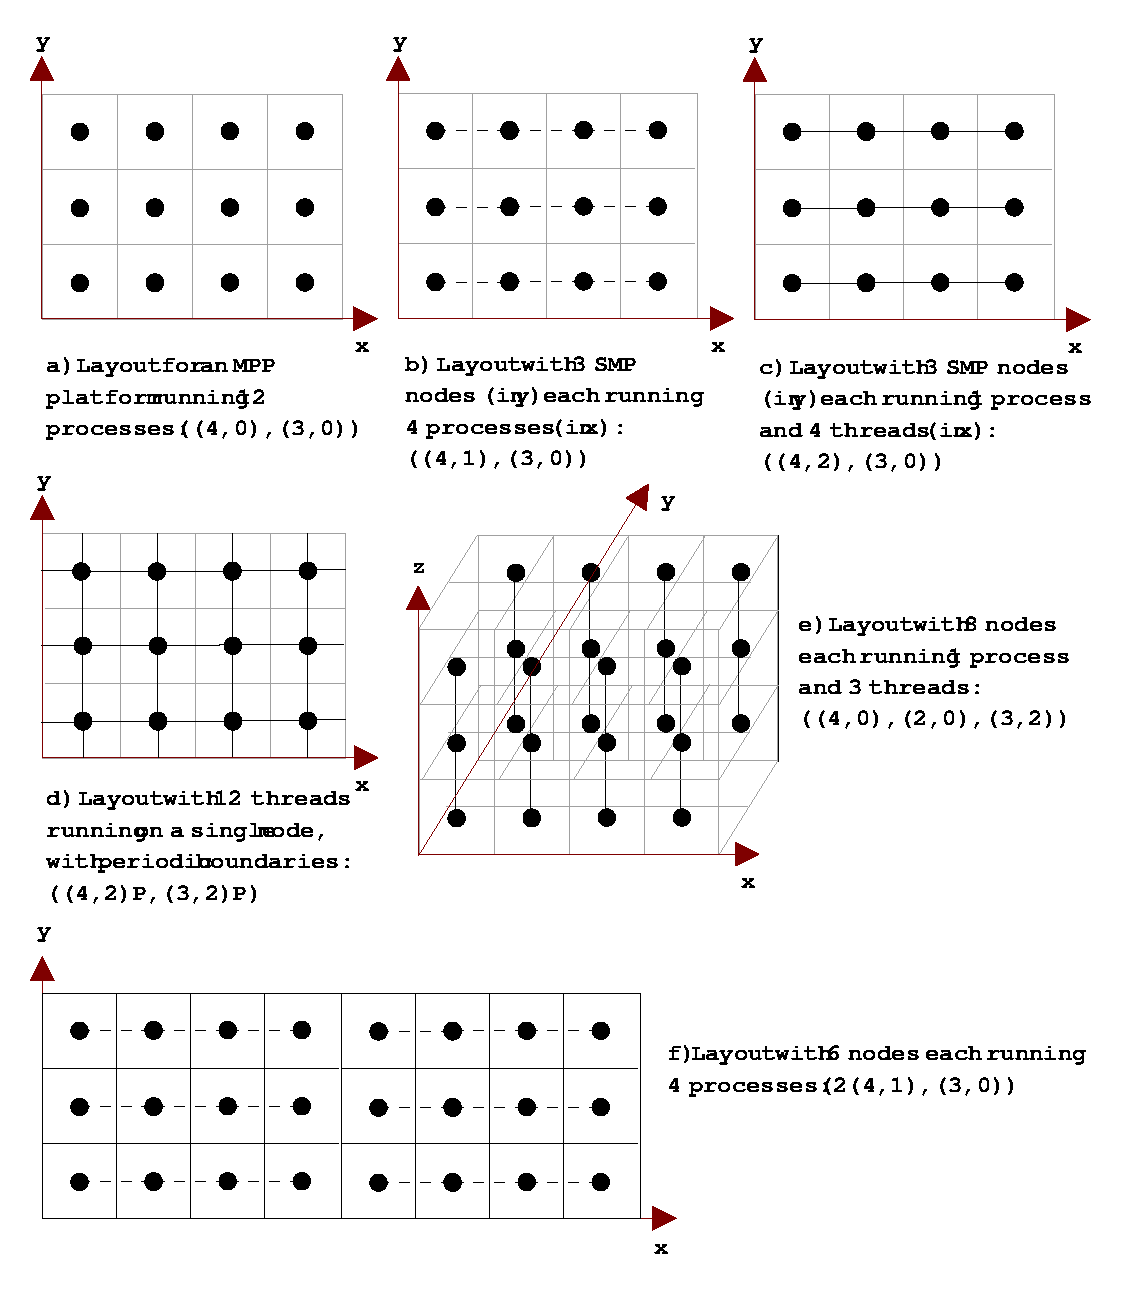
\includegraphics{Layout.eps}}
\end{figure}

When a {\tt Grid} object is defined on a {\tt Layout}, we require that the dimensions 
of the {\tt Grid} align with the dimensions of the {\tt Layout}.  The superimposition
of a {\tt Grid} on a {\tt Layout} is shown in Figure~\ref{fig:gridlayout}.

\begin{figure}
\caption[{{\tt Grid} aligned on a {\tt Layout}}]{The axes of {\tt Grid}s and {\tt Layout}s are aligned.}
\label{fig:gridlayout}
\scalebox{0.7}{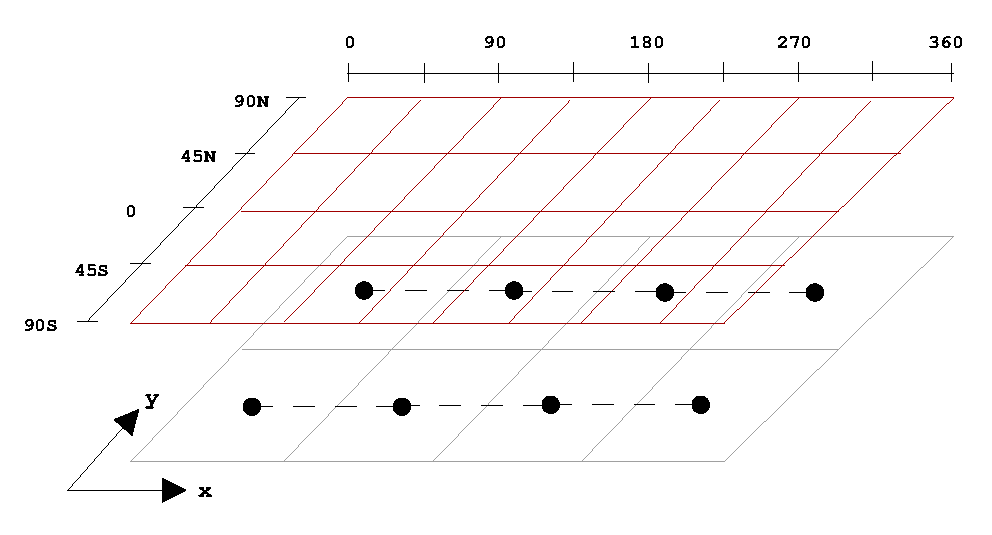
\includegraphics{GridLayout.eps}}
\end{figure}

The user can request system resources either through a simple processor
ID list, or by defining a {\tt Layout}.

\subsection{Class Descriptions}

\subsubsection{Base (ESMF\_Base)}
\label{sec:Base} 
All ESMF objects inherit from an ESMF {\tt Base} class.  
The {\tt Base} class is an abstraction of the data and behavior common to all
classes in the framework.  Some methods and data can be
inherited directly; others are expected to be overloaded and/or overridden by
higher level objects.  {\tt Base} class methods include setting and querying 
attributes, print, validate, read/write, and restart. 

\subsubsection{Attributes (ESMF\_Attr)}
\label{sec:Attr}
{\tt Attribute}s are a list of (name, value) pairs associated with any 
object in the library. The value can be of any data type. 
There are methods for listing, setting, and querying attribute lists.
These methods are expected to be implemented in the {\tt Base} class
and not specialized by higher level objects.

\subsubsection{Machine Model (ESMF\_Machine)} 
\label{sec:machine} 
The {\tt Machine Model} provides a general abstraction of 
key, system specific, features of computer hardware and system software in
the ESMF Programming Model.
This information is used by the framework to 
perform resource allocation, data distribution, and dynamic load balancing.  
The {\tt Machine Model} can be queried for information such as
platform type(s), number of processors per node, number of nodes, 
memory attributes and configuration, processor type and speed,
communication semantics and performance, 
interconnect attributes, and system library availability.
It may optionally may provide quantative information 
on actual bandwidth and latency through active tests.  

\subsubsection{PE List (ESMF\_PEList)}
\label{sec:pelist} 
A {\tt PE List} is a list of physical processor IDs.  It includes a 
unique identifier for each {\tt PE} which may differ from the hardware 
processor ID.  

\subsubsection{Layout (ESMF\_Layout)}
\label{sec:layout} 
A {\tt Layout} describes the topology of a set of {\tt Decomposition 
Elements}.
It is used by any part of the ESMF which needs
to decompose a task/problem/dataset into subsets.
The decomposition must allow for mapping certain subsets onto the
underlying machine model in a preferential way; e.g. keeping
vertical blocks of a 3D decomposition on processors which share
a memory pool.  The user may specify generally which 
dimensions of the {\tt Layout} require the most rapid communication.
A user may also explicitly control the {Layout} by specifying which 
communication mechanisms are preferred for a particular dimension.
The {\tt Layout} may interact with both the {\tt PE List}s
and the {\tt Machine Model} in order to accomplish a preferential
decomposition.

\subsubsection{Basic Communications (ESMF\_Comm)}
\label{sec:basiccomm} 
The {\tt Basic Communication} routines provide a uniform 
interface to the variety of communication mechanisms available
on different hardware platforms.  
The basic functions include methods to send
and receive data, such as scatter, gather, send, receive,
reduction methods such as sum, global min/max, and methods
to synchronize such as barrier. 

\subsubsection{Time Manager (ESMF\_TimeMgr)}
\label{sec:timemgr} 
The {\tt Time Manager} provides general purpose time methods, both
for computing time instants (dates and times) and time intervals
(the difference between 2 time instants).   It also supports 
setting and handling alarm events, either one-shot or repeating.
Supported calendars include Gregorian, Julian, no-leap, 360-day, 
generic, and no-calendar.
Time intervals can range from the very brief -- any rational fraction
of a second -- to geologic time scales.
The {\tt Time Manager} also allows the user to control the format of
time instants and intervals as they are returned.

\subsubsection{Registry (ESMF\_Registry)}
\label{sec:registry} 
A {\tt Registry} maintains a list of (name, ID) pairs per 
namespace.  It supports the many classes in the system which are
required to have unique names, either per address space or over the entire
application.  The {\tt Registry} class provides methods to
create, query, and list namespaces and define their scope.  
Within a namespace it provides methods to
verify a name exists, add a (name, ID) pair,
generate a new unique name, retrieve an ID by name, 
and list existing names.

\subsubsection{Error Handler (ESMF\_Error)}
\label{sec:error} 
The {\tt Error Handler} provides both uniform handling of errors and
a way for users to select how errors will be handled.
An integer error code can be returned from the framework to the
calling code, or the framework can print an error message and exit.
Error messages include information such as the file name, line number, 
and a description of the error.

\subsubsection{Log (ESMF\_Log)}
\label{sec:log} 
The {\tt Log} utility organizes diagnostic output, 
which may be generated in parallel at unpredictable times in
a multiprocessor environment.  It labels the output so that 
searches and filters may be easily constructed.  The quantity of
output is assumed to be moderate to small, i.e. the {\tt Log} 
will not be used to output large streams of numerical model output data.  
It provides methods for writing output and for selecting the
output format, i.e., a single log file vs. a log file per process.

\subsubsection{Diagnostics (ESMF\_Diag)}
\label{sec:diagnostics} 
The {\tt Diagnostic} routines provide assistance with both performance
profiling and code debugging.  Timing routines support measurement
of time intervals at a per-thread granularity around instrumented
sections of code.  Instrumentation links to libraries that can report 
more sophisticated performance statistics if those libraries are available 
on the computing platform.  Debugging routines allow dynamic control over the level
of detail, enabling or disabling of different functional categories,
and assistance with bit-level comparisons for debugging strategies which 
involve running a simulation under differing conditions and
comparing intermediate results.  These routines use methods from
the {\tt Log} class to collect and output results.








